\documentclass[../main.tex]{subfiles}

\begin{document}
In this thesis we studied the required conditions for guiding of high intensity lasers in the LWFA scheme in straight and curved gas--filled capillaries. The curved capillaries are intended to be a medium for composing several acceleration stages to propagate laser pulses over many Rayleigh lengths, in a "fish--bone" scheme.

We demonstrated a working set--up to produce jitter controlled plasma discharges in both straight and curved capillaries, achieving control on the time scale of a few nanoseconds,
\begin{equation*}
    	\tau_\text{jitter}\approx 5\pm 1\si{\ns}.
\end{equation*}
%The primary motivation is to guide a high intensity short laser pulse,
The time window for which optical guiding exists was found to be $\sim$\SI{350}{\ns} after the plasma ignition, and to last
\begin{equation*}
    \Delta t_\text{channel}=50-150\ \si{\ns}.
\end{equation*}
%$$\Delta t_\text{channel}=\SIrange{50}{100}{\ns}.$$
Using a low intensity laser, a maximum radiation transmittance of 6.7 was observed.

A correlation between the applied voltage difference and the radiation transmittance, was observed viz., a higher voltage difference implies a higher transmittance.

Formation of the plasma channel for the straight capillary was cross--checked by spectroscopy measurements. We observed radial parabolic density profile channel with an increase in the electron density of $$\Delta N_e =\SI{0.4e18}{\per\cubic\cm}$$ and radius
$$r_\text{ch}\approx \SI{50}{\um}$$ with on-axis electron density $$N_e(0)=\SI{0.4e18}{\per\cubic\cm}.$$

The mean plasma density across the longitudinal capillary dimension was found to be \SI{2.85e17}{\per\cubic\cm}.

When experimenting with a curved capillary, we couldn't repeat the same demonstration of optical guiding with the oscillator laser pulse--train. The system is jitter--controlled, \textcolor{red}{the plasma does responds to the laser radiation (no transmission in later times) but there is no guiding.}

In future experiments we will check for the guiding  conditions of these gas filled capillaries and explore further the  possibilities of incorporating these capillaries in a laser wakefield electron acceleration scheme. If successful, it would provide a possibility to accelerate electrons to TeV energy levels at distances of tens of meters in comparison to many kilometers in classical accelerators.


%\begin{figure}
%    \centering
%    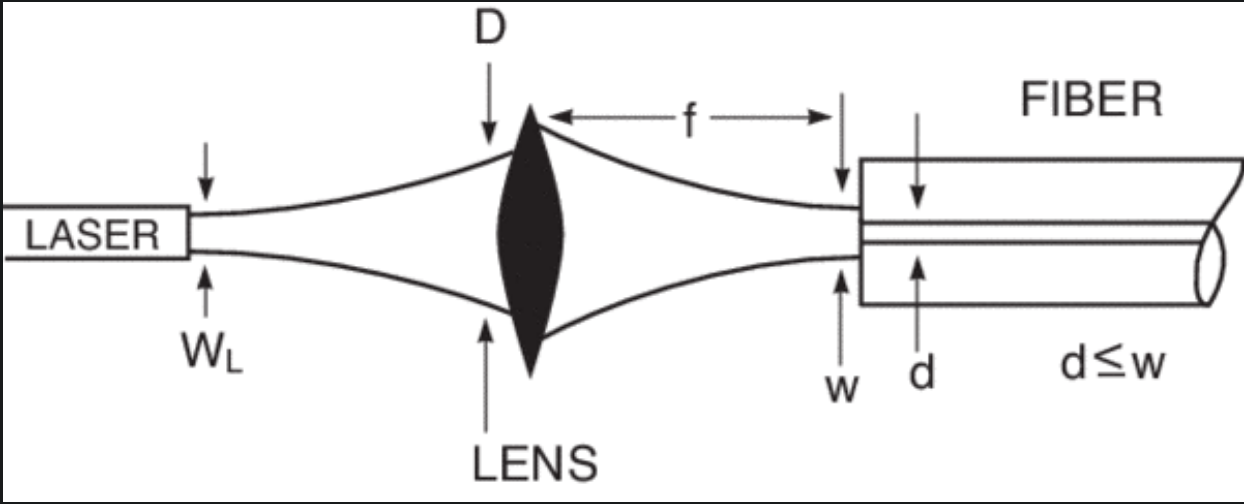
\includegraphics[width=\textwidth]{figures/Curved capillaries/coupling light to fiber.PNG}
%    \caption{\href{https://www.newport.com/t/fiber-optic-basics}{From here.}}
%    \label{fig:fiber}
%\end{figure}

\end{document}